\documentclass[12pt]{article}
\usepackage{tipa}
\usepackage{graphicx}
\usepackage[section]{placeins}
\usepackage{pbox}
\usepackage{lmodern}
\usepackage[math]{cellspace}
\usepackage{caption}
\usepackage{enumerate}
\usepackage{parskip}
\usepackage{framed}
\usepackage{hyperref}
\usepackage{pdfpages}
\RequirePackage{vmargin}		% Force narrower margins
\setpapersize{USletter}
\setmarginsrb{1.0in}{1.0in}{1.0in}{1in}{0pt}{0pt}{0pt}{0in}
\begin{document}
\title{Design Document}
\pagenumbering{gobble}
\setlength{\voffset}{0cm}
\setlength{\hoffset}{0cm}

\includepdf[pages=-]{DesignDocCoverPage.pdf}
\setlength{\voffset}{-2.54cm}
\setlength{\hoffset}{-2.54cm}
\tableofcontents
\clearpage
\pagenumbering{arabic}


\renewcommand{\thefigure}{\arabic{section}.\arabic{figure}}

\section{Executive Summary}
Technology plays an integral part in our daily lives and continues to redefine how we function.  An example of this is the Philips Hue Lights. The Hue Lights are LED lights that can replace any Edison screw light bulb in a home.  These Philips Hue Lights have many different mobile applications for controlling them. These applications can do anything from changing the color and brightness to setting alarms and timers for bulbs. While these applications are useful, they do not do a perfect job. Most applications focus only one a single way to control the bulbs. This means that in order for the user to have a full experience with the bulbs then the user has to switch from one application to another to use the feature unique to each app to control the bulbs. Team Prism will not only fix this issue of having to switch between applications, but also improve it.  This will be done by incorporating the most useful features from the existing applications, improving them, and adding bluetooth position tracking to further automate the Hue Light experience in a home. 
 
A more notable feature will be the ability to synchronize the Hue Lights to music in real time.  This has already been done, but not well. The problem with the existing applications that do it is that there seems to be no rhyme or reason behind how the music is causing the bulbs to change.  We will fix this problem by allowing the user to set rules per bulb as to how each bulb will change to the music. While music synchronization is paramount to this application, it is only the beginning of the story of how this application will change the way people interact with Hue Lights.

There will be many more features other than music synchronization. These features will allow the user to automate the bulbs based off the user's Geolocation, set timers and alarms, and make the bulbs change according to user defined rules.  An example for this would be if the user wakes up at 6am then the Hue Lights will turn on at 5:50am and gradually brighten over a ten minute duration. These are some of many ways that the Hue application will simplify and improve upon the current user experience. 

With all of our features, users will have full control over their Philips Hue Light bulbs from a single application and will no longer have a need to cycle through multiple applications to have the fullest feature experience.  Improving features and making them accessible in a single mobile aplication is not the only way that we will improve the current experience with the Philips Hue Lights. 

In conclusion, our Hue Lights mobile application will improve the way people experience the Hue Lights by letting them have more control over the bulbs than ever before.  With our application there will be no need to have many Hue Lights applications on a single device in order to fully control them. 
\section{Background}
Our inspiration for this project came from the lack of an application that fully encompassed the broad range of features the Hue Light bulbs are capable of. There were several disparate applications that could be combined to create a serviceable controller for the bulbs, but even mixing and matching did not allow the user enough control over the light bulb's behavior. For instance, the Philip's Hue iOS application allows the user to change a light bulb's color and the Ambify by Kai Aras synchronizes the light bulbs to music but this only allows the user to control their light bulbs in a disjointed manner. Our application, however, will allow the user to access these key features in a single application while providing better control over the general workings of the bulbs.

Our goal of a creating the best Hue light mobile application is a lofty one and if done right has the potential to be the most widely used Hue application.  There will be no major need or use for any of the other existing applications after team Prism finishes this application.  Our application will allow more control over the Philip Hue bulbs than any other application and will do so in a easy to use fashion.

\subsection{Required Technology}
We plan to develop an iOS and Android application using Swift and Java respectfully.  Our focus will be on creating a working version in the most recent versions of iOS and Android. There already exists a Phillips Hue API that we will use to control the lights with RESTful JSON messages.  

\subsection{Software/Hardware Requirements}
Our system is going to require a number of hardware devices for testing, all of which team Prism already has on hand.  These will include the mobile devices, network infrastructure, and the Hue Lights themselves. Aside from the mobile devices and the Philips hardware, we plan to encorporated the Estimote bluetooth beacons into our project in a innovative manner.

As for the software side, the software necessary for implementing our project is already part of standard libraries. For example, in pitch detection with real time audio, we will use the native audio processing libraries in the respective platform.  We will also use native libraries for displaying the audio in waveform or we may use the Visualization Toolkit, VTK (\url{http://www.vtk.org/Wiki/VES}) to do our visualizations of the real time audio. On top of that, we plan on using the K-Means clustering algorithm (\url{http://en.wikipedia.org/wiki/K-means_clustering}), which we may or may not need to implement ourselves, to cluster pitches so that we can programmatically assign pitch ranges to particular bulbs. After that, much of our code will rely purely on user interface and backend libraries.  There are also plans to use Estimote bluetooth beacon API to improve the user experience. 


\clearpage

\section{Requirement Analysis}


\subsection{System Architecture}   
%How do these combine together?
%What is the purpose of the server and the database?
%Who commands the light bulbs
%Combine the two mobile sections into 1

\subsubsection*{Hue Lights}
The Hue Lights will be controlled by the Web Server and mobile applications via Philip's Hue Light API.

\subsubsection*{iOS Application}
The Prism project will have an iOS application that will have an intuitive UI for controlling the Hue light bulbs.  The iOS application will interface directly with the Philip's Hue API as well as through the Web Server.

\subsubsection*{Android Application}
The Prism project will have an Android application that will have an intuitive UI for controlling the Hue light bulbs.  The Android application will interface directly with the Philip's Hue API as well as through the Web Server.
\begin{figure}[ht!]
    \centering
    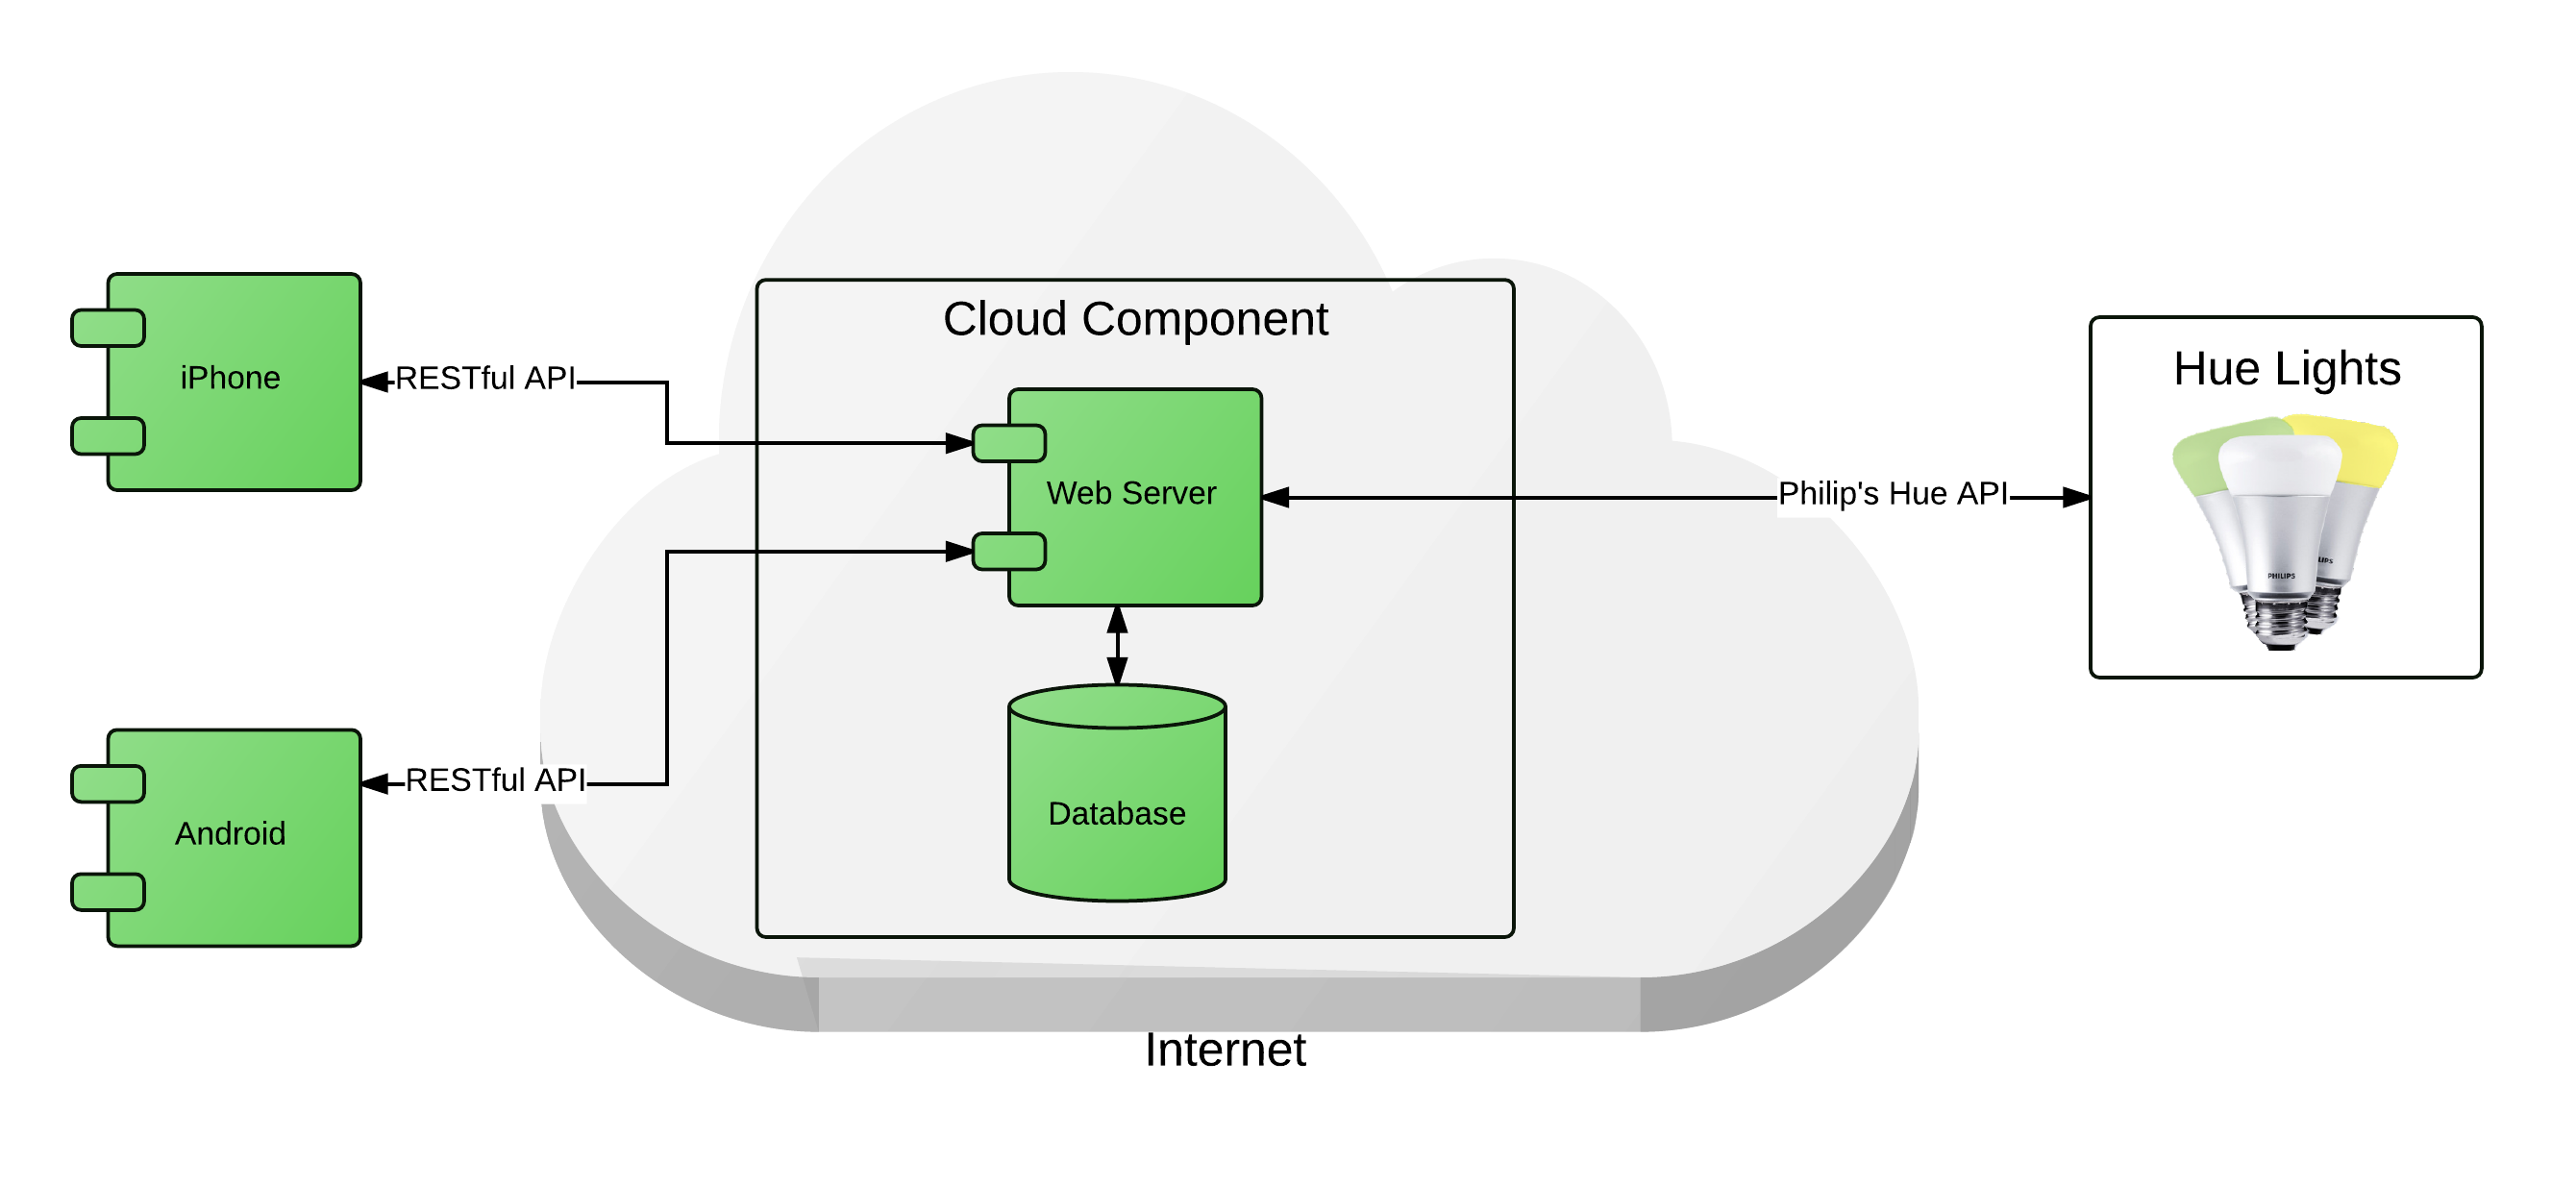
\includegraphics[width=130mm]{System_Architecture_-_System_Architecture.png}
    \caption{System Architecture}
  \end{figure}
\FloatBarrier
\subsection{Personnel}
Each team member will be the lead on specific areas of the system architecture.
\subsubsection*{Trudy Firestone}
Trudy will be focusing on the GUI and backing up Brian on the Android application. She has taken the Android Mobile Application Programming course in Fall of 2014, so she will be well prepared for this responsibility. 
\subsubsection*{Cody Foltz}
Cody's main responsibility is the iOS application.  He has past experience creating applications for other clients and will be able to handle this application.

\subsubsection*{Alma Knudson}
Alma's main responsibilities are the Music Synchronization algorithms, Philip's Hue API interaction for both mobile applications, and the indoor tracking using the Estimote bluetooth beacons. His experience in data mining will allow him to develop sophisticated algorithms to cluster music pitches in real time. 

\subsubsection*{Brian Oh}
Brian's main responsibilities will be developing the Android application. His experience from taking the Android development class will prove to be paramount in his epic journey on this project.

\subsection{System Features}
The features in the system are broken into three sections, bare essentials, planned features, and bells and whistles.  The bare essentials must be finished or the entire system will not work.  The planned features are the features that should be finished by release time while the bells and whistles are the features that would be nice to have before release but are not expected to be finished in time.
\subsubsection*{Bare Essentials}
\begin{itemize}
\item Manual control of a single light bulb
\begin{itemize}
\item Toggle a single light on/off
\item Change a single light bulb's color
\item Adjust the brightness of a single light bulb
\item User will be able to control the bulb through the LAN and through the server
\end{itemize}




%Do we still handle this in a clever way?
\item User Accounts
\begin{itemize}
\item User will be able to authenticate to the server
\item Allow or deny access to a bulb
\item Guest account
\end{itemize}

\item Alarms
\begin{itemize}
\item Lights turn on/off at a specific time
\item Can be set to gradually turn off or on
\end{itemize}
\item Timers	
\begin{itemize}
\item Turns light off after X amount of minutes
\item Can be set to gradually turn off light
\end{itemize}

\item Manually control groups of light bulbs
\begin{itemize}
\item Assign bulbs to groups
\item Manually control a group of bulbs
\end{itemize}
\item User Controls
\begin{itemize}
\item Users will be able to enable and disable features
\item User preferences are saved on the server
\end{itemize}

\item Music Synchronization
\begin{itemize}
\item When audio is sensed by the mobile device's microphone then the Hue bulbs will change color and brightness to that audio
\end{itemize}
\end{itemize}

\subsubsection*{Planned Features}
\begin{itemize}
\item Dynamic Lighting
\begin{itemize}
\item Sunset - Lights dim as sun comes up
\item Sunrise - Lights brighten as sun goes down
\item Weather - Lights brighten when weather blocks out the sun
\end{itemize}


\item User Access controls
\begin{itemize}
\item User can be restricted from specific features
\end{itemize}
	
\item Cycle colors automatically
\begin{itemize}
\item Set a bulb to cycle through specific colors over a time period
\item Set color, duration, brightness, and transition speed
\end{itemize}

\item Voice Commands
\begin{itemize}
\item Toggle individual bulbs on and off by bulb name- "Night stand bulb, on"
\item Toggle group of bulbs on and off by group name- "Kitchen bulbs, off"
\item Change the color of individual and/or group of bulb- "Kitchen bulbs, blue"
\end{itemize}


\item Music Synchronization
\begin{itemize}
\item Real time audio will be presented on the GUI in a pitch wave.  The user will be able to select a pitch range that will determine the range of pitches that a particular light bulb will change to. These settings will then be able to be saved as a theme.  This allows for the creation of several themes that can be reused later.
\end{itemize}


\item Geolocation
\begin{itemize}
\item Prism will allow users to set a geographical location (called GeoFencing) that notify the server when the user enters or exits that location.  The server will then be able to modify lights based on the user entering or exiting that location. 
\end{itemize}
\end{itemize}

\subsubsection*{Bells and Whistles}
\begin{itemize}
\item Voice Commands
\begin{itemize}
\item Voice commands to enable/disable a specific feature
\item Change color and brightness via voice commands
\end{itemize}
	
\item Advanced Music Synchronization
\begin{itemize}
\item To make this Music Synchronization feature truly advanced the pitches will be clustered programmatically, and Prism will provide a default theme for music based off of these pitch clusterings. This will require minimal modifications to our Mock UI for this feature, but will require a significant amount of algorithm work.
\end{itemize}

\item Share User Created Data
\begin{itemize}
\item User will be able to share groups, themes, schedules and other feature settings with other users
\end{itemize}

\item Schedules
\begin{itemize}
\item Be able to create a daily schedule for when the lights should be on/off, brightness, and color
\item Ability to save the schedule for reuse
\end{itemize}


%Do we need this?
\item Light sensor
\begin{itemize}
\item User will be able to add optional light sensors for ultimate automated light control
\end{itemize}
\end{itemize}
%Temporary clearpage so we can see how long it is
\clearpage

\section{Software Engineering Tools and Techniques}
\subsection{Agile Vs. Waterfall}
As our main software engineering process, we've chosed to use agile development. Each week will represent a single sprint. These small sprints will allow us to remain on track to complete our project. Initially, it's unlikely that we will have a finished version of Prism at the end of each sprint, but we still plan to set goals and review the sprint for these initial weeks. Once we have our bare essentials completed for both of our mobile platforms, we should be able to complete an improved product at the end of each sprint which we can test over the course of the following sprint. This will allow us to focus on maintaining a polished project while we continue to add features.
\subsection{Versioning, Bug Tracking, and Documentation}
As a team, we decided we wanted to have our coding skill be something we could be proud to present to others.  We thought the best way to present our code would be on a public site such as GitHub.  We found that in addition to the normal public git repository, GitHub also has bug tracking, pull requests (request for peer review), and a wiki.  We plan to use all of these features not only to help ourselves stay on track but to allow everyone the chance to see how the project evolves through out the senior year.  

Our team is committed to using git and we plan to have at least one other member of the team peer review code prior to merging that code into the master branch.  Directly after that review, we'll update the wiki with any useful information and close out any issues that have been resolved.  This will allow us to stay up to date with documentation and project issues while hopefully lowering the amount of potential bugs in the project.

\subsection{Testing}
\begin{itemize}
\item Family and friends to test just by using the application
\item Automated Unit tests on the server side
\item UI testing for Android and iOS
\item testing each other's features
\item document testing from the beginning
\item try to automate as much testing as possible
\end{itemize}
\subsection{Team Communication and Meetings}
\begin{itemize}
\item group texts
\item google hangouts
\item git issue tracking
\item version one
\item calling for urgent needs
\item team meeting agenda --each person talks for a few minutes describing what they've been doing, updates team on what they've accomplished the previous week and what they'll accomplish the following week. Discuss roadblocks teh person is having.
\item Meeting before class each Monday and Wednesday.
\item Retrospective-what we did last week that was bad and how we can improve it each Monday.
\end{itemize}
\clearpage



\section{Appendix}
\setcounter{figure}{0}
  \subsection{Use Cases}
  \begin{samepage}
  \begin{framed}
    \textbf{Use Case 1}\\
    %Clarify how connect to server works
    \textbf{Title}: Initial Setup\\
    \textbf{Short Description}:  The Actor will set up the Hue light application for first time use.  \\
    \textbf{Actor}: Homeowner \\
    \textbf{Precondition}: Have Philip's Hue lights, mobile device, and optional Estimote beacons. \\
    \textbf{List of Steps}:
    \begin{enumerate}
      \item Replace incondecent bulbs with Hue bulbs
      \item Place Estimote beacons in each room or every 25 feet (beacons are optional)
      \item Install app on mobile device
      \item Open app
      \item App will then auto locate Bridge
      \item Authenticate app with Bridge by following on screen instructions
      \item Name lightbulbs
    \end{enumerate}
    \textbf{Related UI}: See Figure \ref{fig:settings} 
  \end{framed}
\end{samepage}

\begin{samepage}
  \begin{framed}
    \textbf{Use Case 2}\\
    \textbf{Title}: Change Single Light Bulb's Color\\
    \textbf{Short Description}: The Actor changes the color of a single Hue light bulb.\\
    \textbf{Actor}: Homeowner \\
    \textbf{Precondition}: Actor is logged into app \\
    \textbf{List of Steps}:
    \begin{enumerate}
      \item Select bulb
      \item Open bulb settings in manual control
      \item Change color of bulb
    \end{enumerate}
    \textbf{Related UI}:  See Figure \ref{fig:home} and Figure \ref{fig:singleControl} 
  \end{framed}
\end{samepage}

\begin{samepage}
  \begin{framed}
    \textbf{Use Case 3} \\
    \textbf{Title}: Group bulb setting \\
    \textbf{Short Description}: The Actor can group Hue light bulbs together and control them as if they are a single Hue light bulb. \\
    \textbf{Actor}: Homeowner \\
    \textbf{Precondition}: Actor is logged into app \\
    \textbf{List of Steps}:
    \begin{enumerate}
      \item Open group settings
      \item Name group
      \item Add bulbs to group
      \item Save group
    \end{enumerate}
    \textbf{Related UI}:  See Figure \ref{fig:home} and Figure \ref{fig:singleControl}. In Figure \ref{fig:home}, a group is created by dragging a lightbulb onto another. 
  \end{framed}
\end{samepage}

\begin{samepage}
  \begin{framed}
    \textbf{Use Case 4} \\
    \textbf{Title}: Schedule \\
    \textbf{Short Description}: The actor sets up a schedule for their lightbulbs. \\
    \textbf{Actor}: Homeowner \\
    \textbf{Precondition}: Actor is logged into app and has used app for at least one day \\
    \textbf{List of Steps}:
    \begin{enumerate}
      \item Navigate to schedule menu
      \item Copy previous day's schedule to today
      \item Add an additional scheduled item through the calendar menu
      \item Select device to be scheduled
      \item Apply rule, color, etc. through manual control.
      \item Save schedule
    \end{enumerate}
    \textbf{Related UI}:  See Figure \ref{fig:schedule} and Figure \ref{fig:singleControl}
  \end{framed}
\end{samepage}

\begin{samepage}
  \begin{framed}
    \textbf{Use Case 5} \\
    \textbf{Title}: Music Light Control \\
    \textbf{Short Description}: The actor syncs their music and lightbulbs by the selecting a predefined music synchronization theme.\\
    \textbf{Actor}: Homeowner \\
    \textbf{Precondition}: Actor is logged into app \\
    \textbf{List of Steps}:
    \begin{enumerate}
      \item Play music that is audible to the microphone on device
      \item Navigate to the Music Light Control Menu
      \item Select predetermined music synchronization theme
      \item Watch bulbs change to the music
    \end{enumerate}
    \textbf{Related UI}: See Figure \ref{fig:musicThemes} 
  \end{framed}
\end{samepage}

\begin{samepage}
  \begin{framed}
    \textbf{Use Case 6} \\
    \textbf{Title}: Music Synchronization Theme Creation \\
    \textbf{Short Description}:  Actor creates a new music theme that will control the lights in real time based on the music playing. \\
    \textbf{Actor}: Homeowner \\
    \textbf{Precondition}: Actor is logged into app \\
    \textbf{List of Steps}: 
    \begin{enumerate}
        \item Navigate to Music Light Control Menu
        \item Add new theme
        \item Select range of pitches for each bulb
        \item Set colors that a bulb can show
        \item Save theme
    \end{enumerate}
    \textbf{Related UI}:  See Figure \ref{fig:musicThemes} and Figure \ref{fig:musicRules} and Figure \ref{fig:musicColors} 
  \end{framed}
\end{samepage}

\begin{samepage}
  \begin{framed}
    \textbf{Use Case 7} \\
    \textbf{Title}: Custom Automation Rule \\
    \textbf{Short Description}: Actor creates an automated task \\
    \textbf{Actor}: Homeowner \\
    \textbf{Precondition}: Actor is logged into app \\
    \textbf{List of Steps}:
    \begin{enumerate}
        \item Navigate to automation rules
        \item Select create new ``Cause Effect" rule
        \item Name the rule
        \item Set the ``Cause" to some event. (ie. specific time, enter room, dish washer finished, arrive home, etc.)
        \item Set the ``Effect" to be an event that the Actor would like to happen. (ie. turn on lights, start to brew coffee, notify Actor, turn on hot tub, etc.)
        \item Save the rule
        \item Enable the new rule
    \end{enumerate}
    \textbf{Related UI}:  See Figure \ref{fig:singleControl}, Figure \ref{fig:rules}, Figure \ref{fig:newRule}, and Figure \ref{fig:newCauseEffectRule}
  \end{framed}
\end{samepage}

\begin{samepage}
  \begin{framed}
    \textbf{Use Case 8}\\
    \textbf{Title}: Enable Predetermined Automation Tasks For a Bulb\\
    \textbf{Short Description}: User wants to enable a predetermined automation task for a bulb\\
    \textbf{Actor}: Homeowner \\
    \textbf{Precondition}: Actor is logged into app \\
    \textbf{List of Steps}:
    \begin{enumerate}
      \item Navigate to rules
      \item Select bulb
      \item Turn on predetermined feature
    \end{enumerate}
    \textbf{Related UI}:  See Figure \ref{fig:singleControl} and Figure \ref{fig:rules} 
  \end{framed}
\end{samepage}

\begin{samepage}
  \begin{framed}
    \textbf{Use Case 9}\\
    \textbf{Title}: Color Cycle Setting\\
    \textbf{Short Description}: Actor can make a rule to have a bulb cycle through a set of colors over time. \\
    \textbf{Actor}: Homeowner \\
    \textbf{Precondition}: Actor is logged into app \\
    \textbf{List of Steps}:
    \begin{enumerate}
     \item Navigate to automation rules
     \item Select create new color cycle rule
     \item Name the color cycle rule
     \item Select bulbs
     \item Set the starting color
     \item Set the brightness of the first color
     \item Set the amount of time before transitioning to the next color
     \item Repeat steps 5 through 7 for each color to be included in the cycle
     \item Save the rule
     \item Start rule
    \end{enumerate}
    \textbf{Related UI}:  See Figure \ref{fig:singleControl}, Figure \ref{fig:rules}, Figure \ref{fig:newRule}, Figure \ref{fig:newCycleColorRule}, and Figure \ref{fig:addColorCycle}
  \end{framed}
\end{samepage}



\subsection{UI Sketches}
  \begin{figure}[ht!]
    \centering
    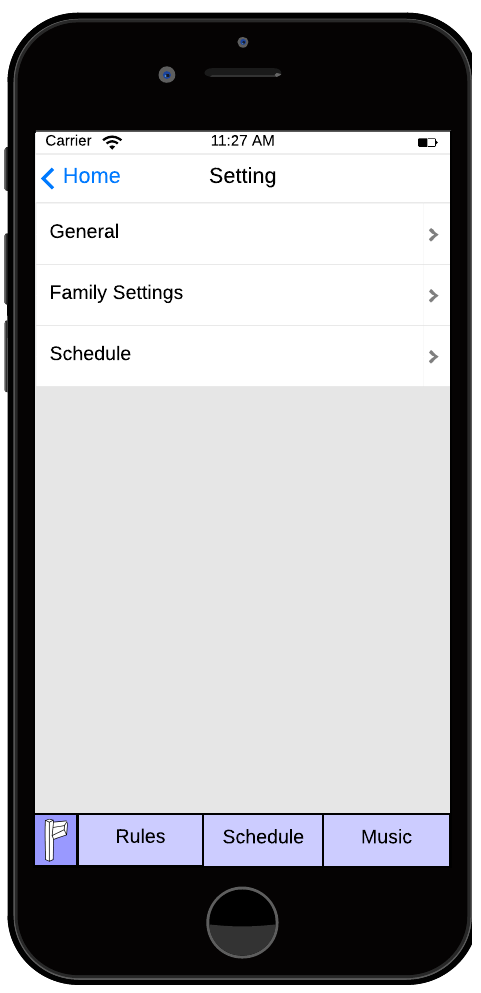
\includegraphics[width=50mm]{Settings.png}
    \caption{General Settings}
    \label{fig:settings}
  \end{figure}
  
  \begin{figure}[ht!]
    \centering
    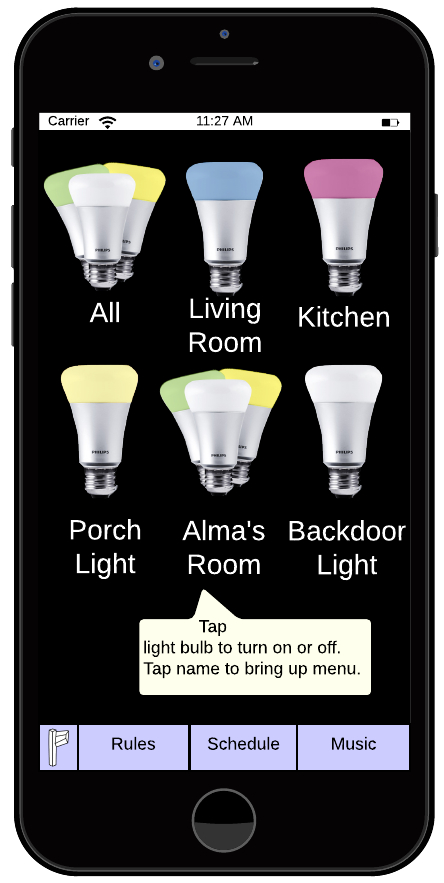
\includegraphics[width=50mm]{Home.png}
    \caption{Home Screen}
    \label{fig:home}
  \end{figure}
  
  \begin{figure}[ht!]
    \centering
    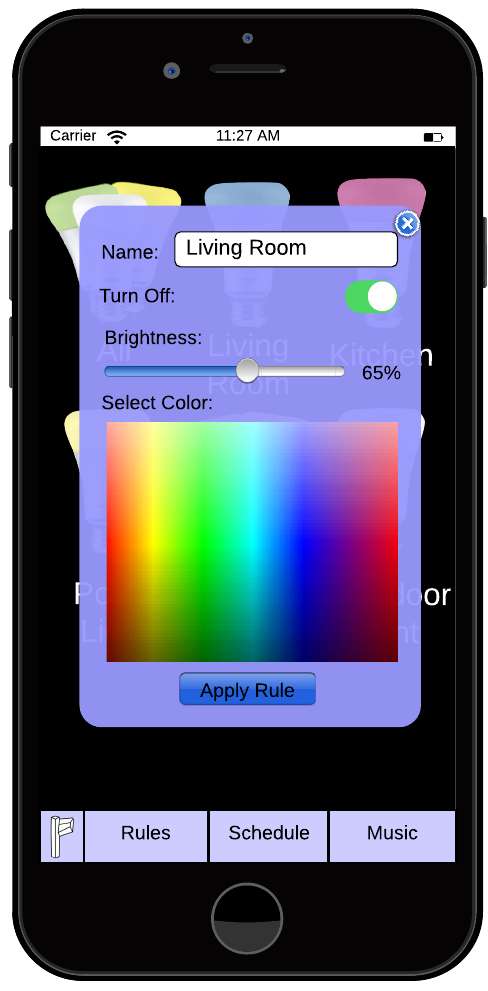
\includegraphics[width=50mm]{ManualControl.png}
    \caption{Manual Control}
    \label{fig:singleControl}
  \end{figure}
  
  
  \begin{figure}[ht!]
    \centering
    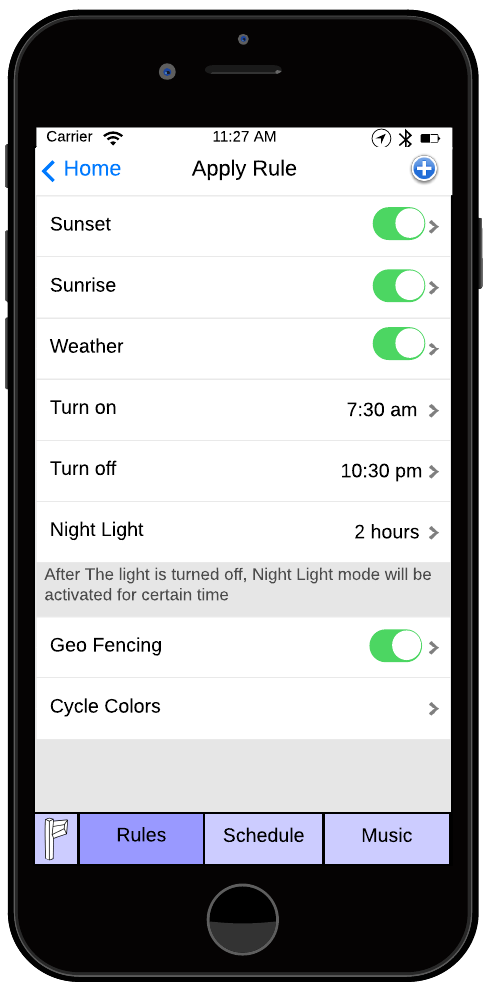
\includegraphics[width=50mm]{ApplyRule.png}
    \caption{Rules}
    \label{fig:rules}
  \end{figure}
  
  \begin{figure}[ht!]
    \centering
    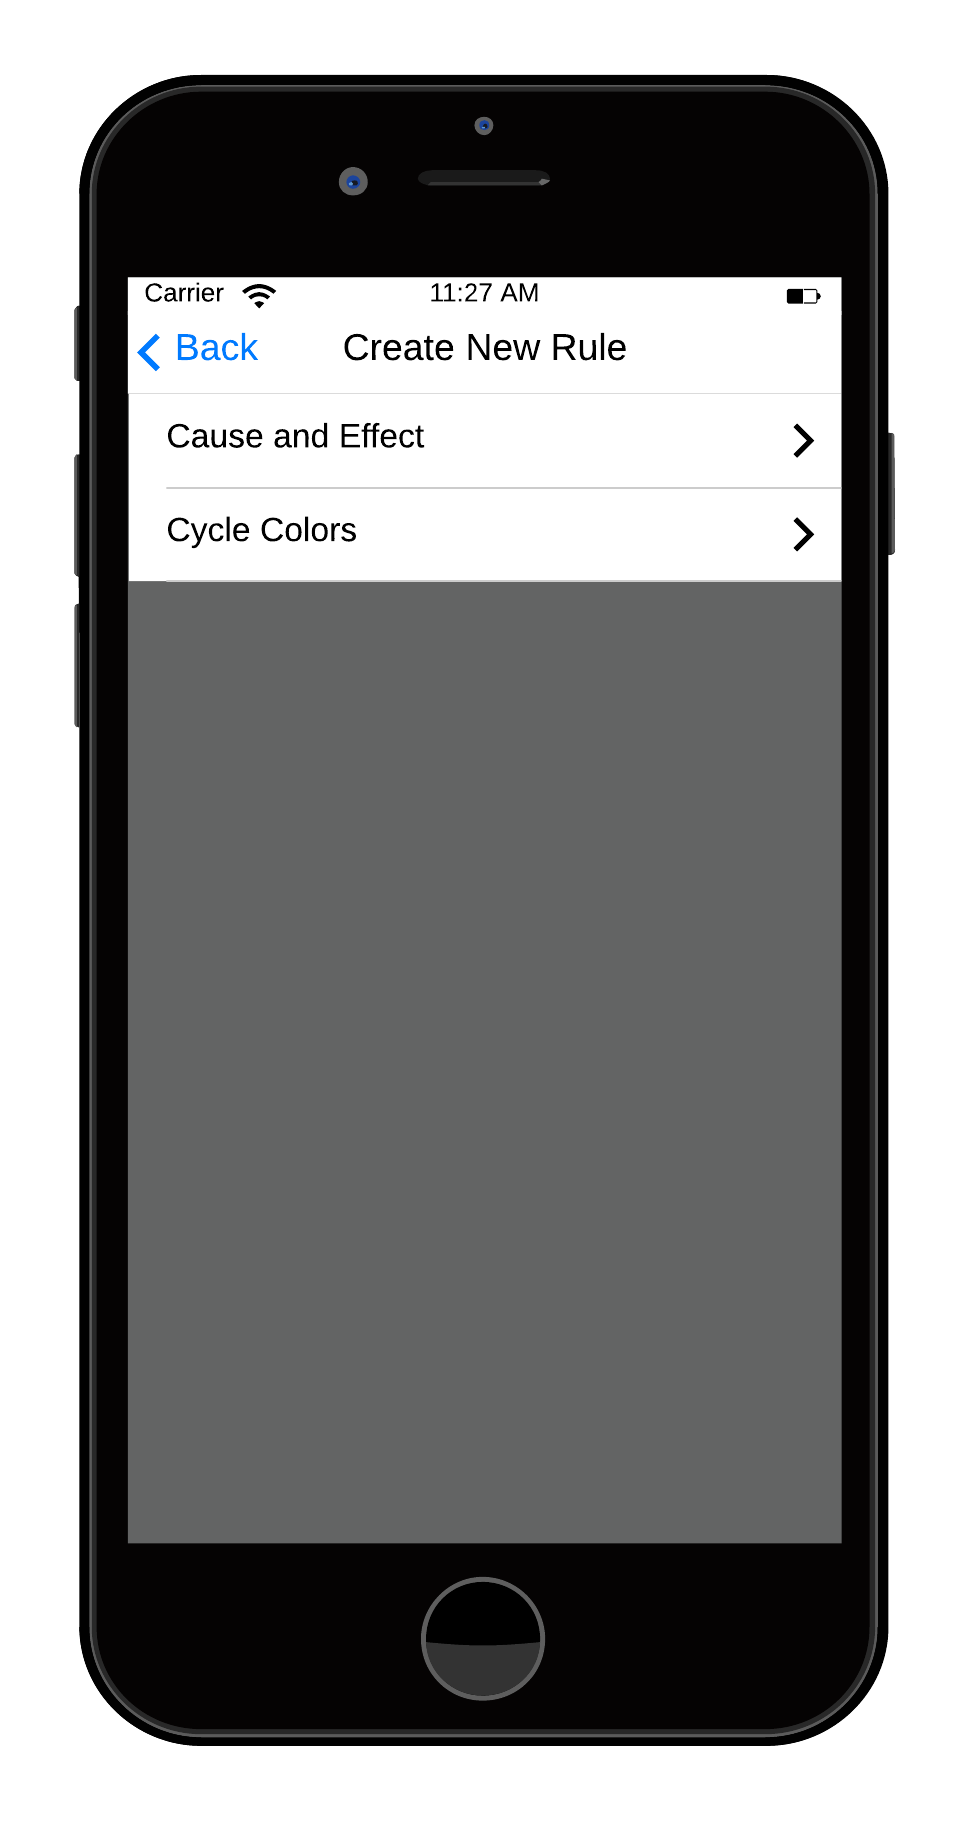
\includegraphics[width=50mm]{Create_Rule.png}
    \caption{Create New Rule}
    \label{fig:newRule}
  \end{figure}
  
  \begin{figure}[ht!]
    \centering
    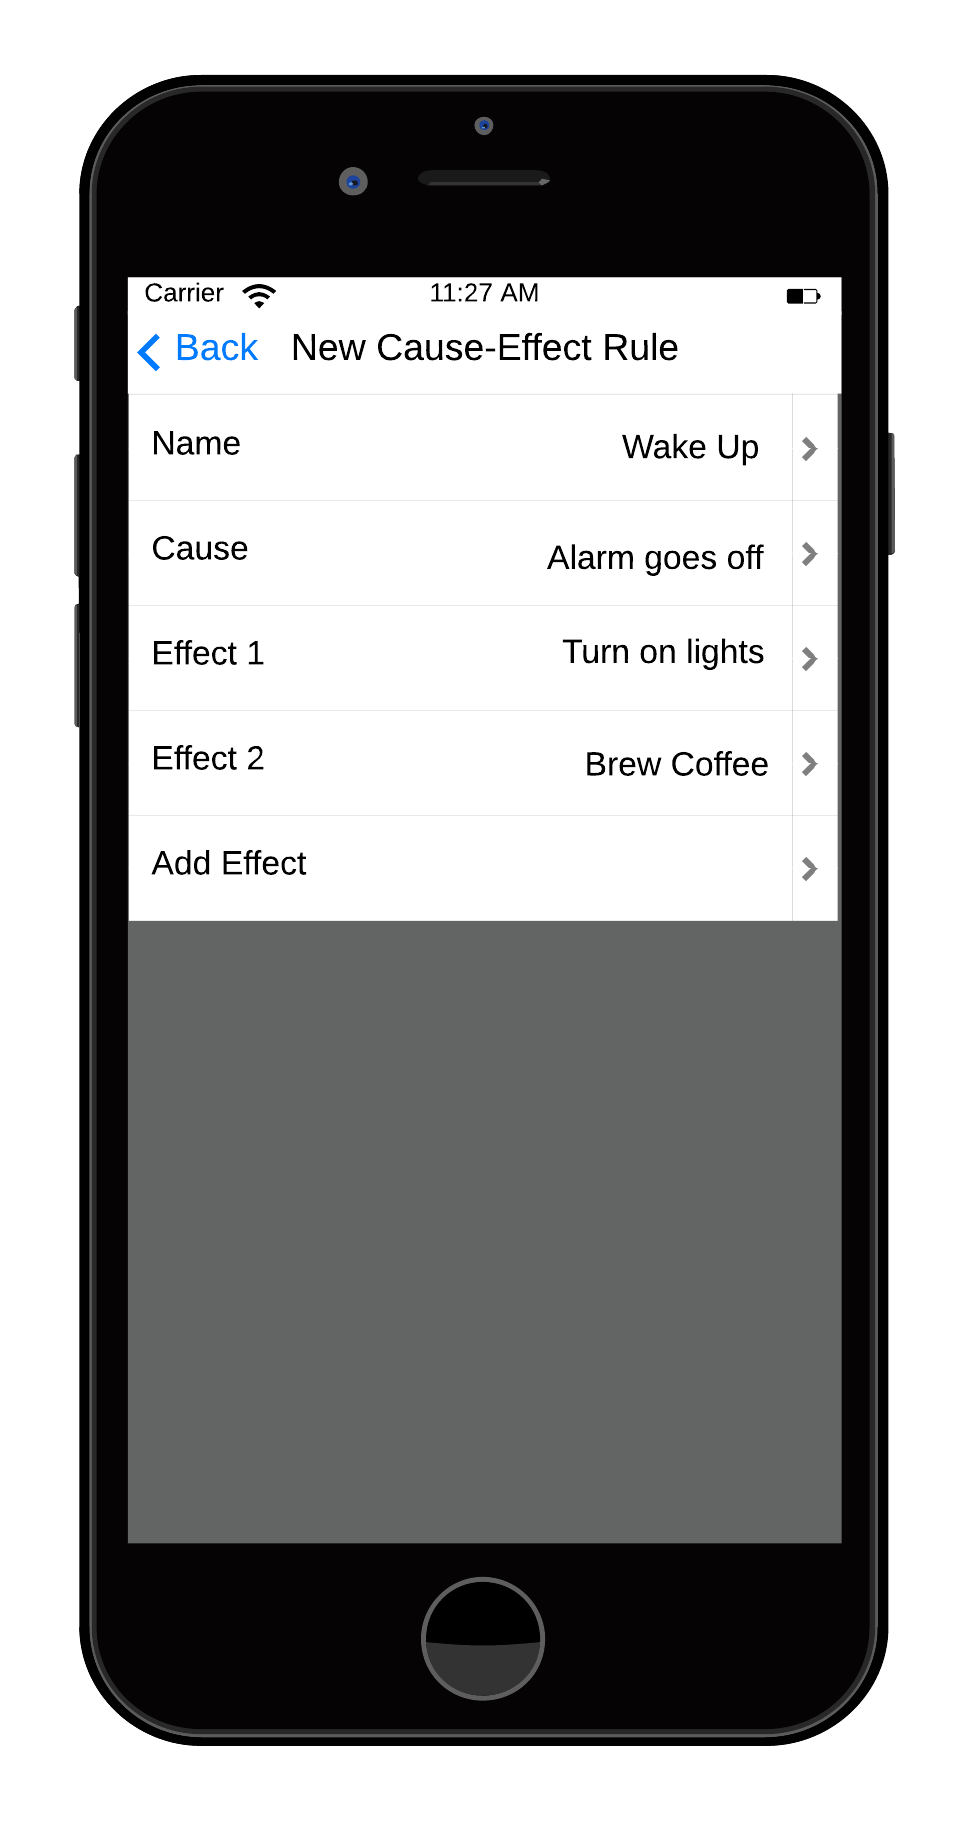
\includegraphics[width=50mm]{CauseEffect.png}
    \caption{Create New Cause-Effect Rule}
    \label{fig:newCauseEffectRule}
  \end{figure}
  
  \begin{figure}[ht!]
    \centering
    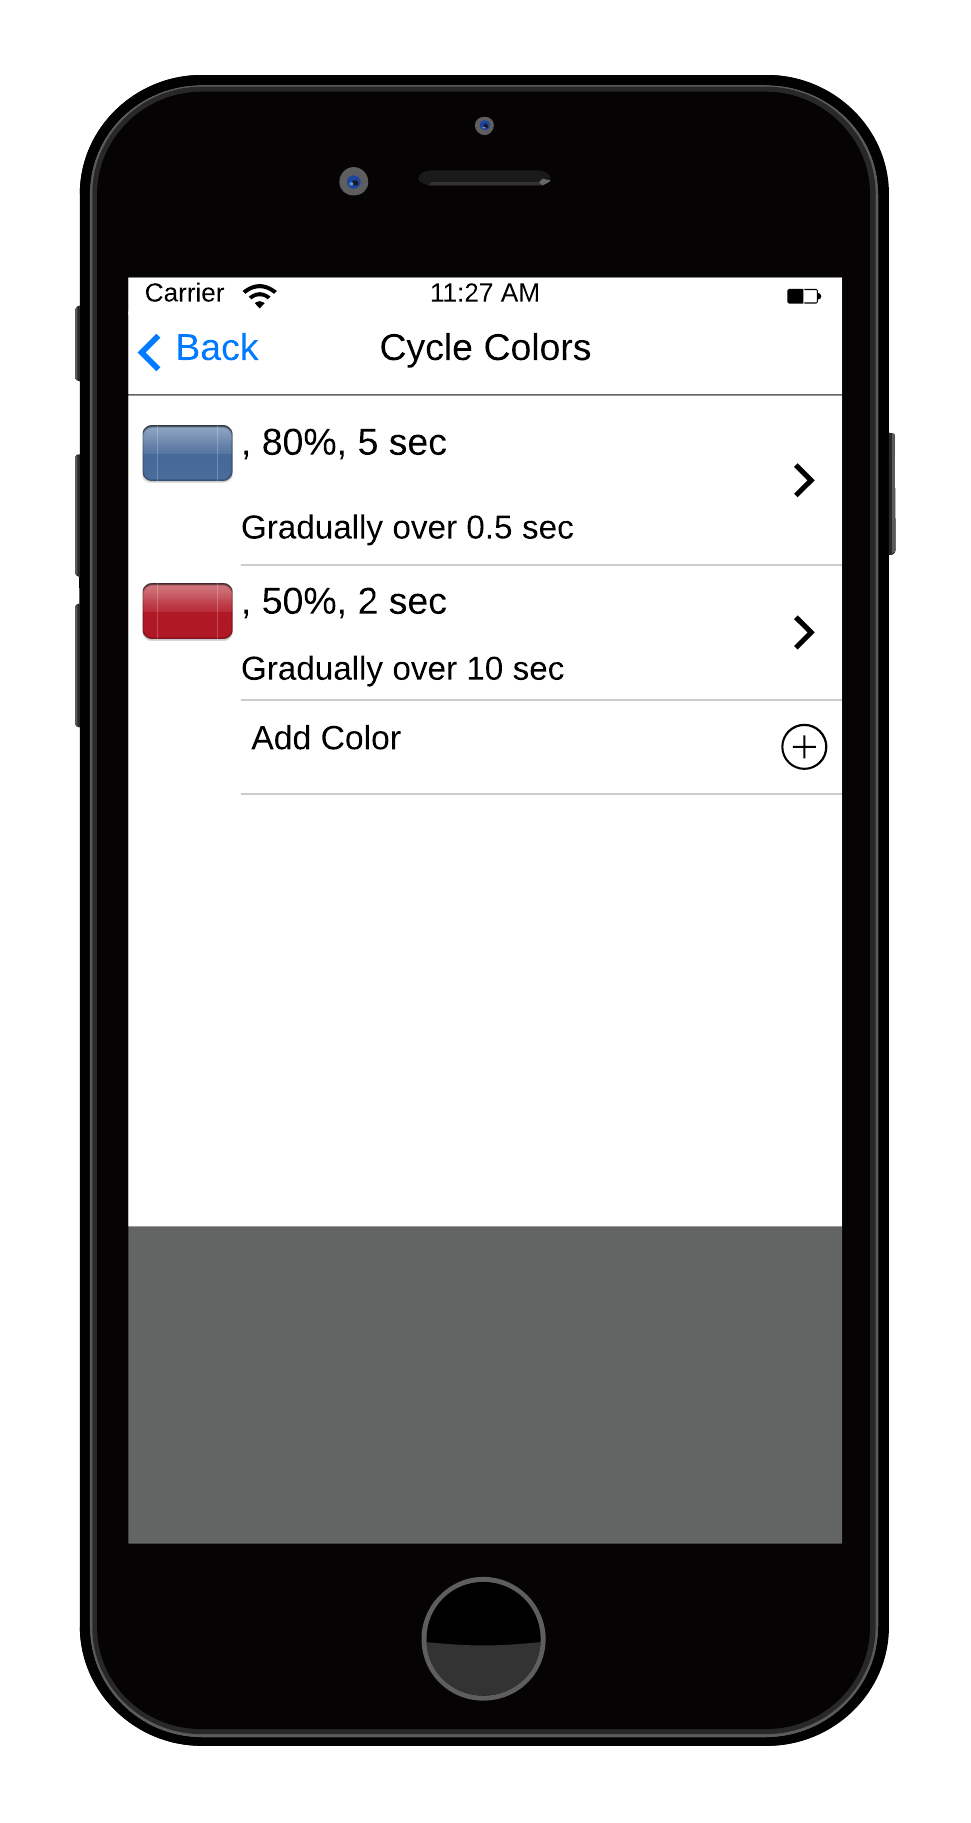
\includegraphics[width=50mm]{Cycle_Colors.png}
    \caption{Create New Cycle-Color Rule}
    \label{fig:newCycleColorRule}
  \end{figure}
  
  \begin{figure}[ht!]
    \centering
    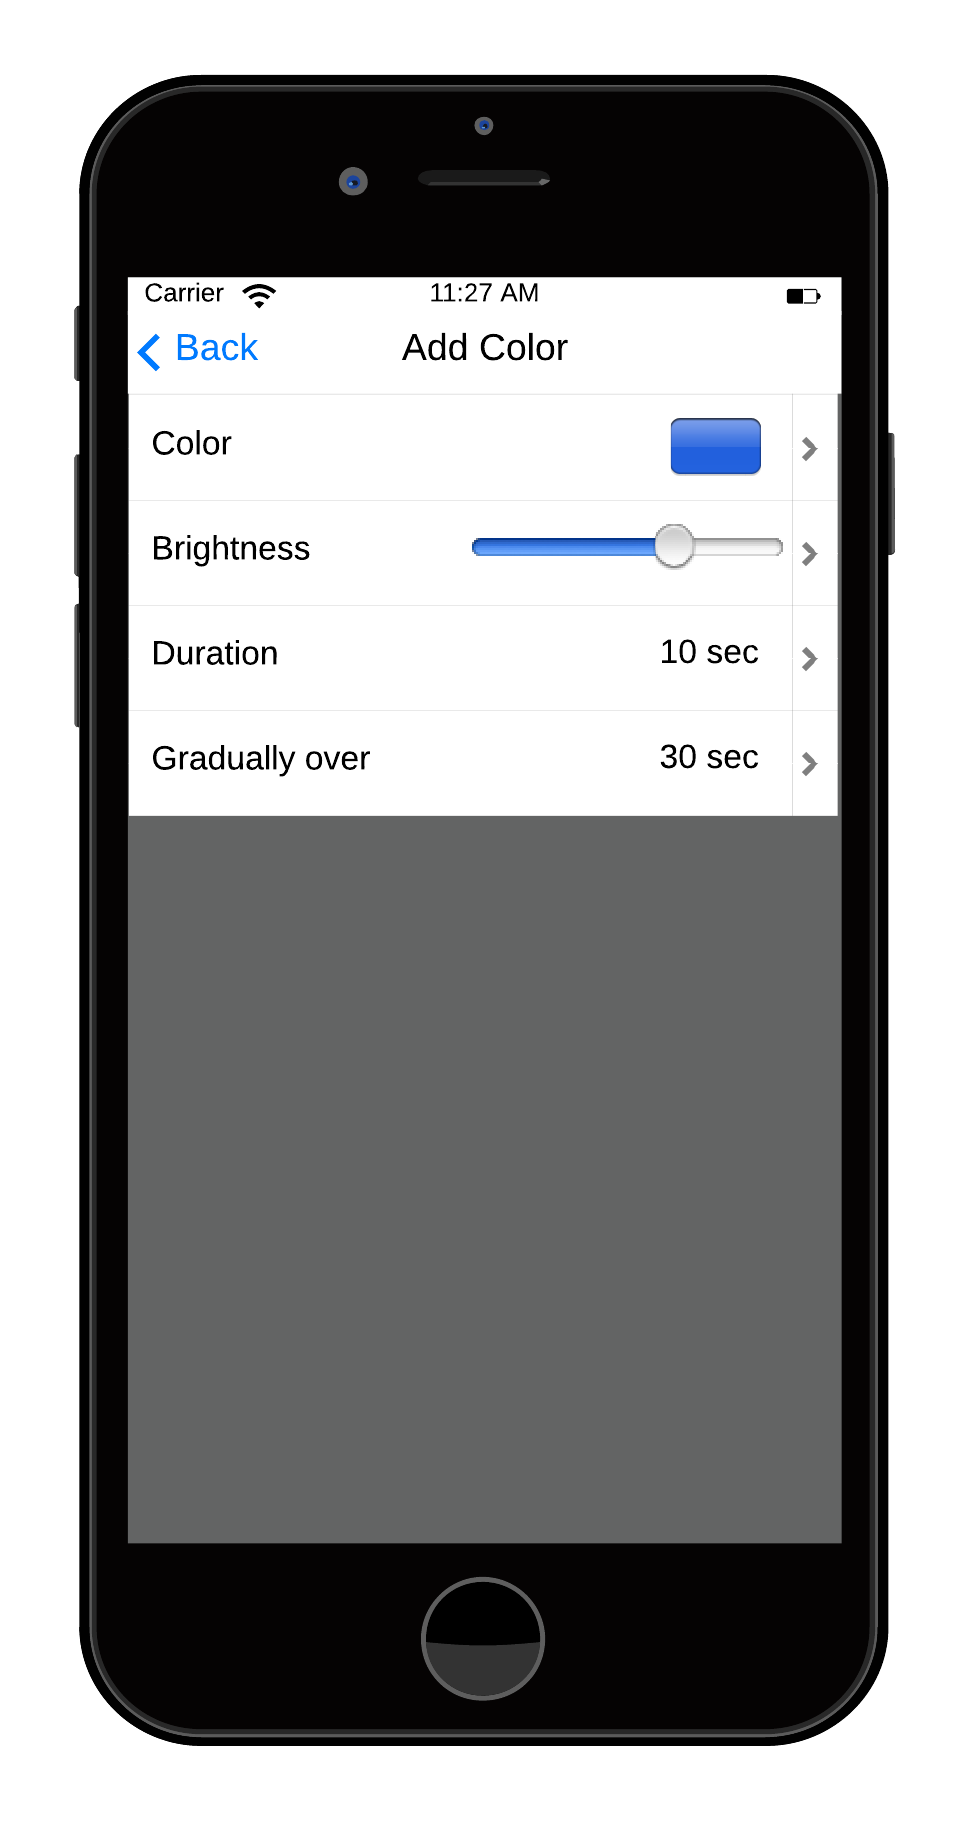
\includegraphics[width=50mm]{Add_Color.png}
    \caption{Add Color to Color Cycle}
    \label{fig:addColorCycle}
  \end{figure}
  
  \begin{figure}[ht!]
    \centering
    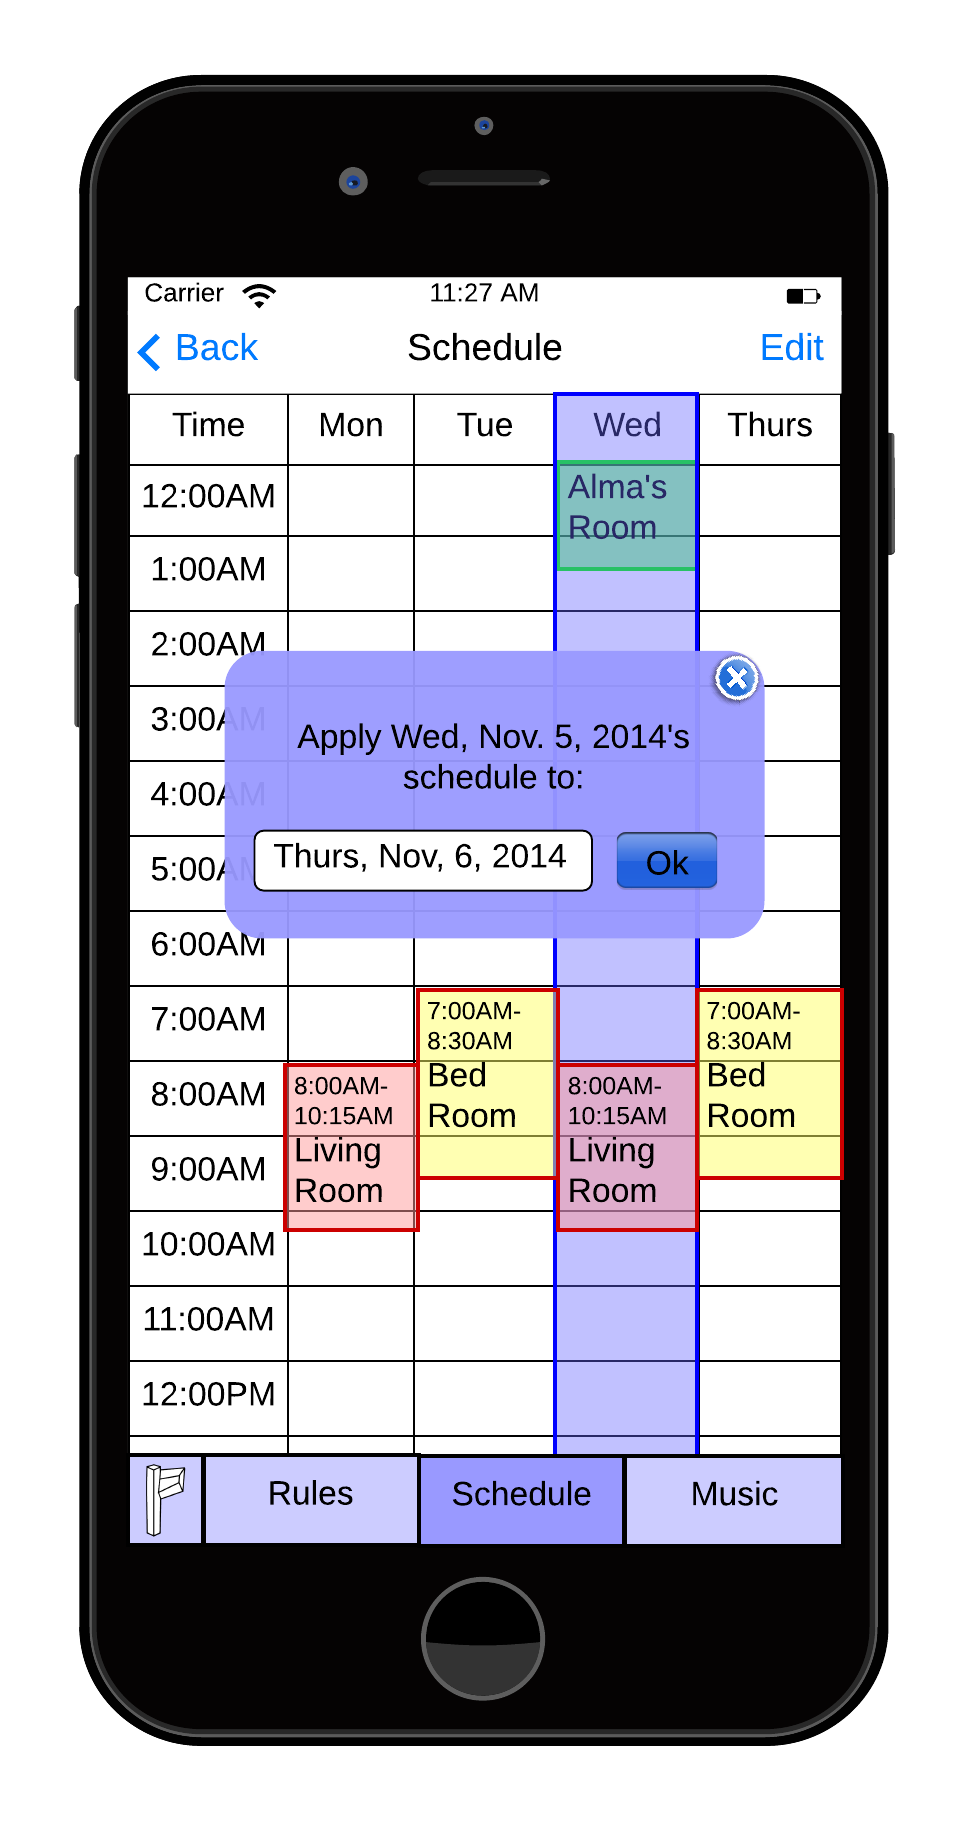
\includegraphics[width=50mm]{Schedule.png}
    \caption{Schedule}
    \label{fig:schedule}
  \end{figure}
  
  \begin{figure}[ht!]
    \centering
    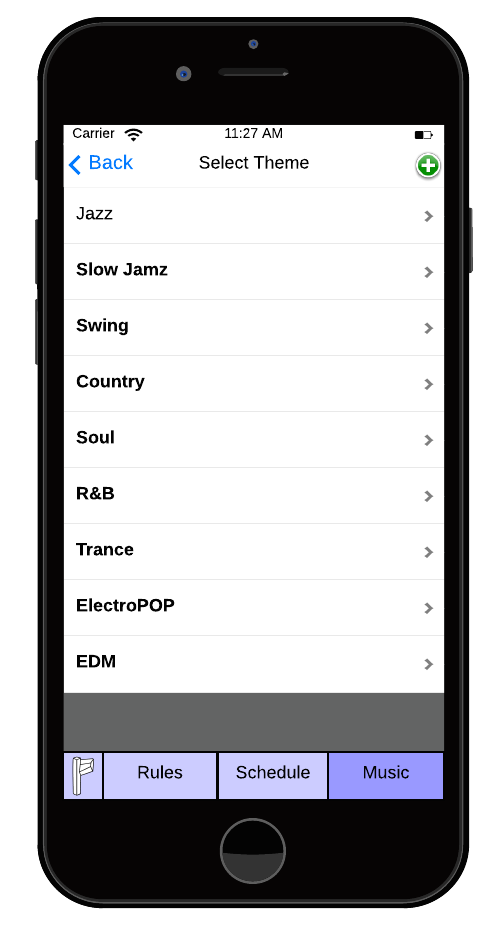
\includegraphics[width=50mm]{iPhone_music_theme.png}
    \caption{Music Themes}
    \label{fig:musicThemes}
  \end{figure}
  
  \begin{figure}[ht!]
    \centering
    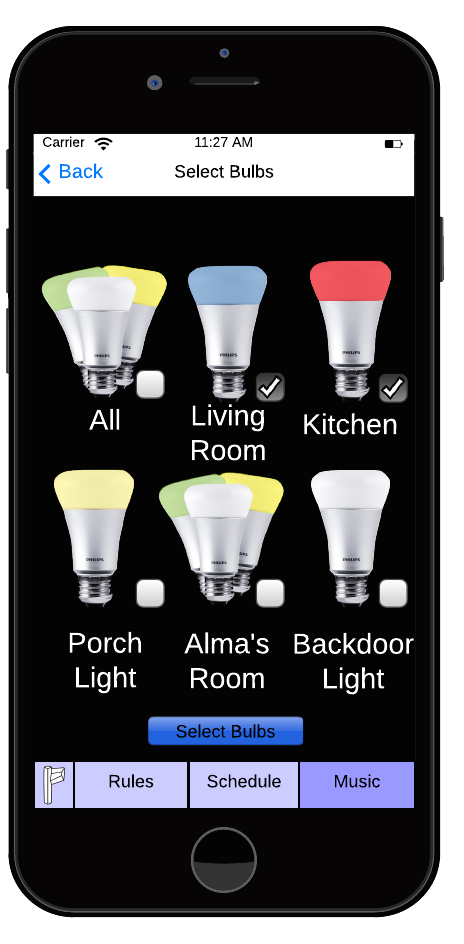
\includegraphics[width=50mm]{iPhone_music_select_bulb.png}
    \caption{Bulb Selection Screen}
    \label{fig:bulbSelectionScreen}
  \end{figure}
  
  \begin{figure}[ht!]
    \centering
    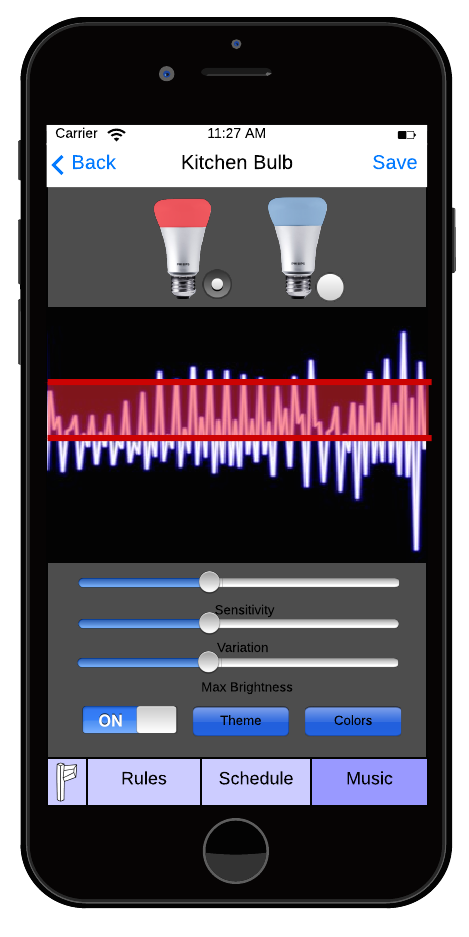
\includegraphics[width=50mm]{iPhone_music_main.png}
    \caption{Music Rules Screen}
    \label{fig:musicRules}
  \end{figure}
  
  \begin{figure}[ht!]
    \centering
    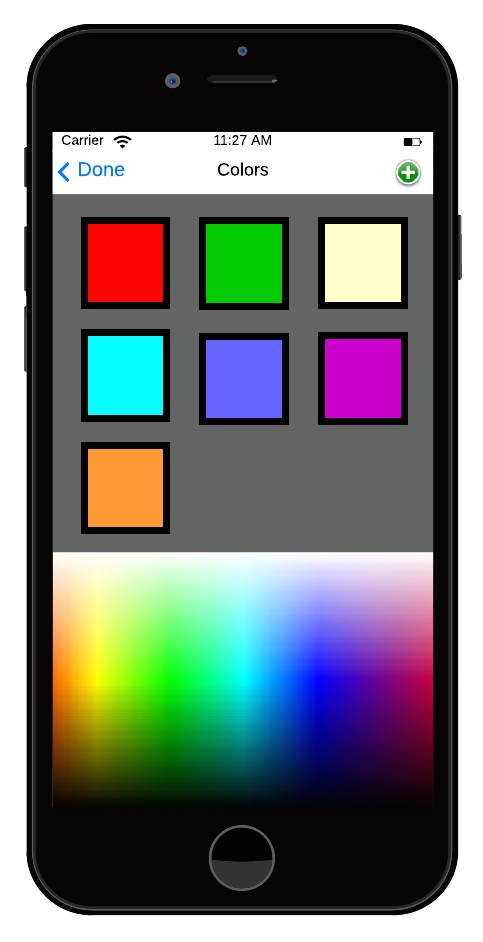
\includegraphics[width=50mm]{iPhone_music_color.png}
    \caption{Music Colors Screen}
    \label{fig:musicColors}
  \end{figure}
\end{document}